\section{Анализ предметной области}

В данной части будет проанализирована предметная область автоматической проверки чертежей на ошибки оформления, рассмотрена нормативная база, выделены основные ошибки в оформлении и приведены методы анализа ошибок.

\subsection{Понятие чертежа и его регламентирование}
% Чертежом называют документ, содержащий изображения предметов: деталей, узлов, машин и т.д., необходимых для ее изготовления.


% На международном уровне функции стандартизации выполняет серия стандартов
% ISO~\cite{iso}. Несмотря на схожесть, ГОСТ и ISO имеют ряд специфических различий в деталях оформления,
% что создает необходимость в разработке средства, проверяющее заданные правила.

В рамках единой системы конструкторской документации чертёж определяется как конструкторский документ,
содержащий изображение изделия и иные данные, необходимые для его изготовления и контроля.
Согласно ГОСТ 2.102~\cite{gost-2-102}, чертежи подразделяются на несколько видов:
\begin{itemize}
    \item чертёж детали;
    \item сборочный;
    \item габаритный;
    \item монтажный;
    \item теоретический.
\end{itemize}

Каждый вид чертежа регламентирован в зависимости от назначения и стадии разработки изделия.
Основные требования к оформлению и содержанию чертежей устанавливаются межгосударственными стандартами ЕСКД или международными ISO~\cite{iso}


\subsection{Классификация ошибок в инженерных чертежах}

Ошибки в чертежах часто носят системный характер. Среди наиболее распространённых можно выделить несколько категорий.
\begin{enumerate}
    \item оформление основной надписи;
    \begin{itemize}
        \item неправильное оформление главной надписи;
        \item отсутствие или неверное заполнение обязательных полей;
        \item использование нестандартных размеров штампа;
        \item нарушение шрифта или размера текста;
    \end{itemize}
    \item оформление надписей, текста и шрифтов;
    \begin{itemize}
        \item использование шрифта отличного от указанного в ГОСТ 2.304~\cite{gost-2-304};
        \item несоответствие высоты букв требованиям;
        \item грамматические ошибки;
        \item нарушение правил штриховки;
    \end{itemize} 
    \item нарушения при нанесении размеров;
    \begin{itemize}
        \item дублирование размеров;
        \item отсутствие необходимых размеров для однозначного изготовления детали
        \item отсутствие стрелок на концах размерных линий;
        \item отсутствие единиц измерения;
        \item неправильное расположение размерных и выносных линий;
    \end{itemize} 
    \item семантические ошибки и логические противоречия;
    \begin{itemize}
        \item наличие нескольких взаимно противоречивых проекций одной и той же детали;
        \item несоответствие между изображением детали и её техническими требованиям;
        \item неправильное применение условных обозначений;
    \end{itemize}

    % \item нарушение при оформлении видов и чертежей
    % \begin{itemize}
    %     \item отсутствие или неправильное оформление рамки поля чертежа;
    %     \item нарушение размеров полей;
    %     \item размещение чертежа за границами установленного поля;
    % \end{itemize} 
    % \item ошибки в формате и рамке;
    % \begin{itemize}
    %     \item отсутствие обозначений разрезов;
    %     \item нарушение правил штриховки.
    % \end{itemize} 
\end{enumerate}

Анализ этих типов ошибок является важным, поскольку он определяет набор правил, которые должна проверять автоматизированная система.

\subsection{Разделение ошибок на формальные и семантические}
При анализе нарушений требований к оформлению чертежей можно выделить два кардинально разных класса ошибок: формальные и семантические.
Формальные ошибки обусловлены несоответствием чертежа, чётко сформулированным правилам стандартизации.
Такие ошибки характеризуются высокой степенью формализуемости: их можно выразить в виде логических предикатов над данными чертежа, что делает их пригодными для автоматической проверки.

Семантические ошибки связаны с некорректностью содержания или логическими противоречиями.
Они не всегда нарушают стандарт, но при этом содержат недочёты, приводящие к невозможности однозначной интерпретации чертежа.
К примеру, можно выделить следующие ошибки:
\begin{itemize}
    \item указание несуществующего материала детали;
    \item несоответствие формы детали её функциональному назначению;
    \item несоответствие разреза реальности. 
\end{itemize}

Выявление семантических ошибок требует контекстного понимания проекта.
В текущей момент автоматизация их обнаружения ограничена уровнем технологий и остаётся предметом исследований в области искусственного интеллекта.
Таким образом, текущие системы автоматизированной проверки в первую очередь ориентированы на выявление формальных ошибок.

\subsection{Стандартный вид системы}

Современные системы автоматизированной проверки конструкторской документации на соответствие требованиям стандартов оформления,
несмотря на различия в реализации, обладают схожей модульной структурой.
Такая архитектура обусловлена общими задачами: загрузка данных, нормализация, проверка чертежа на ошибки оформления и представление результатов пользователю.
Типовая система представлена следующими ключевыми компонентами на рисунке~\ref{scheme_validation_system}:

\begin{figure}[H]
	\centering
	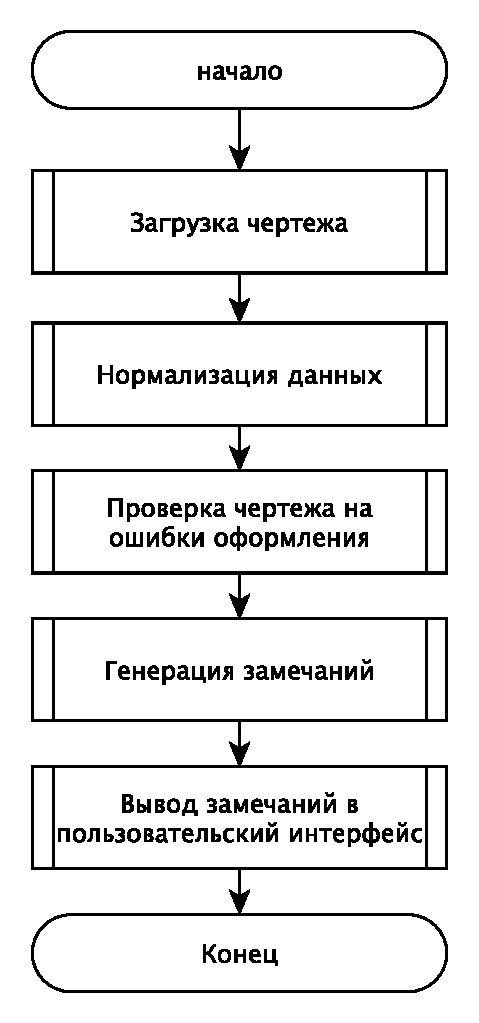
\includegraphics[width=0.35\textwidth]{diag/03-001.pdf}
	\caption{Схема реализации системы автоматизированной проверки чертежа на ошибки оформления}
	\label{scheme_validation_system}
\end{figure}

\subsection{Загрузка чертежей и вывод полученного результата}
Сервисы по нахождению ошибок в оформлении чертежей отличаются между собой системой ввода, вывода и нахождения ошибок, именно об этих различиях пойдет речь в этой подглаве.

\subsubsection{Системы встроенные в САПР} 

Поскольку САПР не предназначены для разработки программных модулей, то некоторые из них имеют специальные библиотеки подпрограмм для взаимодействия --- API,
используя которые, сторонние программы могут обращаться к элементам САПР, создавать, редактировать геометрическую модель, открывать и записывать
файлы, управлять окнами и пр. С помощью API плагин может получить информацию о модели, так, как она хранится в САПР.
За счёт этого исключаются проблемы, связанные с некорректными данными

При использовании API САПР вывод возможен сразу в пользовательский интерфейс системы, например с помощью всплывающих окон.

\subsubsection{Загрузка векторного файла}

Векторный файл --- файл, сформированный множеством геометрических примитивов, объединённых математическими соотношениями.
Каждый объект в векторном формате задается в виде математической функции, поэтому данные формат устойчив к изменению размеров.

Анализ векторных файлов позволяет системе автоматизированной проверки чертежей напрямую извлекать геометрические данные ---
координаты точек, параметры линий, дуг, типы линий, текстовые аннотации и другую информацию.
Кроме того использование векторных файлов, исключает ошибки, связанные с разрешением, шумом, артефактами сжатия или неточностями OCR.

К важным примуществам данного метода можно отнести снижение зависимости системы от API конкретных САПР.
Это обеспечивает платформенную независимость и повышает переносимость системы.
\subsubsection{Загрузка растрового изображения}

В отличие от векторных форматов, растровые данные не содержат структурированной информации о геометрии и тексте,
поэтому их анализ требует методов компьютерного зрения и OCR для извлечения примитивов, надписей, рамки и штампа.
При этом точность зависит от качества изображения, а использование нейросетей снижает детерминированность результата.

\subsection{Методы анализа чертежа на ошибки оформления}
\subsubsection{Алгоритмические проверки}

В современных САПР реализованы функции, обеспечивающие выполнения требований ГОСТ и ЕСКД при разработке конструкторской документации.
Набор функций обеспечивает: автоматическое проставление размеров, номеров позиций, обозначений видов, сечений и т.д.
Эти проверки носят алгоритмический характер и реализуются с помощью формализованных условий --- предикатов,
которые однозначно определяют соответствие конкретного элемента чертежа требованиям стандарта.

% \subsubsection{Сравнение с эталоном}

% Метод автоматизированной проверки чертежей на основе чертежа с разметкой~\cite{marked-method}.
% Эталон создаётся в САПР: пользователь должен выделить контролируемые объекты, добавляет маркеры в виде выносок с текстом, а также использует фигуры-заместители, если нужных фигур нет в САПР.
% Система строит эталонную модель и при проверке ищет соответствующие элементы на входном чертеже и сравнивает их, применяя геометрические преобразования.

\subsubsection{Использование машинного обучения}

Современные достижения в области искусственного интеллекта открывают новые возможности для автоматизированной
проверки чертежей на ошибки оформления. Нейронные сети, способны обучаться на больших наборах чертежей и выявлять отклонения от установленных стандатов.

Одним из ключевых подходов является применение свёрточных нейронных сетей (CNN), которые эффективно извлекают пространственные признаки из изображений чертежей:
геометрические формы, линии, шрифты, размерные обозначения, масштабы и взаимное расположение элементов.
После извлечения признаков система сравнивает их с эталонными шаблонами, соответствующими конкретным стандартам~\cite{ai-method}. Такой подход позволяет автоматически выявлять ошибки оформления — например, неверное начертание штриховки, нарушение масштаба или отсутствие необходимых надписей.

Дополнительно, для анализа текстовой информации, содержащейся на чертеже, могут использоваться
модели обработки естественного языка (NLP).

\section*{Вывод}
В данной части была проанализирована предметная область автоматической проверки чертежей на ошибки оформления, рассмотрена нормативная база, выделены основные ошибки в оформлении и приведены методы анализа ошибок в оформлении чертежей.
 
\clearpage